\documentclass{article}
\usepackage{microtype}
\usepackage{graphicx}
\usepackage{subfigure}
\usepackage{booktabs}
\usepackage{hyperref}
\newcommand{\theHalgorithm}{\arabic{algorithm}}
\usepackage[accepted]{icml2018}
\icmltitlerunning{Numeral Algebra Final Project}

\begin{document}

\twocolumn[
\icmltitle{\textbf{Numerical Algebra Final Project:} \\
    A Numerical Method Solving Anisotropic Poisson Equations}
\begin{icmlauthorlist}
\icmlauthor{Li Ziyao, 1500017776}{}
\end{icmlauthorlist}
\icmlkeywords{PCG, V-Cycle, Poisson Equation, Numerical Algebra}
\vskip 0.3in
]

\begin{abstract}
The main task of this project is to solve the Anisotropic Poisson equation by transforming the original problem into a linear equation using discrete differential approximations. Different methods have been attempted solving the linear equation with massive size, including direct Gauss elimination and Preconditioning Conjugate Gradient (PCG) with V-Cycle preconditioner using either Symmetric Line Gauss-Seidel Iterative Method or Symmetric Point Gauss-Seidel Iterative Method as smoother. Other methods, such as ordinary Conjugate Gradient Methods are also attempted.

Despite the optimization adopted according to the structure of A, Gauss elimination method is too complex to solve the problems with greater size, since it somehow breaks the sparsity of the original matrix in the elimination process. PCG performs better, and adopting Line G-S iterative method as the smoother both computes and converges faster than adopting Point G-S iterative method.
\end{abstract}

\section{Introduction}

The target anisotropic Poisson equation is described as follows:
\begin{displaymath}
  \left\{
    \begin{array}{ccl}
      -u_{xx}-\epsilon u_{yy} &=& f \\
      u|_{\partial \Omega} &=& 0 \\
      (x,y)\in \Omega &:=& (0,1)\times(0,1)
    \end{array}
  \right.,
\end{displaymath}
where $f$ is a given function.

By dividing the original region $\Omega$ into $N \times N$ grids and applying a discrete differential approximation, the original equation can be transformed into a linear equation $Au=f$, where A is a $((N-1)^2 \times (N-1)^2)$ square matrix, u, a $((N-1)^2 \times 1)$ vector, is the numerical solution of the original problem, i.e. the function values on grid points, and f is the given function values in the corresponding form (Detailed description is in the Appendix 1).

The problem is that with $N$ growing up, the size of the problem becomes $N^4$ (the number of elements in A). However, due to the special structure of A, optimizations can be adopted to reduce the complexity.

To solve the linear equation, different methods are attempted, including a Gauss elimination method and a PCG method with a V-Cycle as the preconditioner. The following sections describe the designs and the results of different methods.

\section{Gauss Elimination Method}

Using direct Gauss elimination method to solve the problem including two steps: first implementing an LU decomposition of the matrix A, and then solving two triangular linear equations $Ly=f$ and $Ux=y$. Both steps can be optimized according to the structure of A, for A is a band-width matrix with $bandwidth=2N-1$.

During the LU decomposition process, it is easy to find that only elements in a sub-matrix way smaller than expected is actually altered. Therefore, the total times of addition is reduced from $O(N^6)$ to $O(N^4)$. And similar optimization is available solving triangular linear equations, reducing the complexity from $O(N^6)$ to $O(N^3)$.

However, despite the optimization available, the algorithm is still time-costly since the process of LU decomposition somehow breaks the sparsity of the original A. Elements of the original A distributes only in 5 diagonal and sub-diagonals, but the elements of L and U filled up the entire band-width. This is unavoidable taking any form of Gauss eliminations.

The running time, $l^2$ norm of error and $l^2$ norm of residuals are shown in Table~\ref{tab1}, where
\begin{eqnarray*}
  Error &=& ||u_{calc}-u_{true}||_2/N \\
  Residual &=& ||f-A*u_{calc}||_2/N
\end{eqnarray*}

\begin{table}[t]
\caption{The results of direct Gauss eliminations optimized with band-width information (N=64).}
\label{tab1}
\vskip 0.15in
\begin{center}
\begin{small}
\begin{sc}
\begin{tabular}{lrrr}
\toprule
$\epsilon$ & Time (s) & Error & Residual  \\
\midrule
$10^0$ & 9.50 & $1.00 \times 10^{-4}$ & $2.96 \times 10^{-12}$ \\
$10^{-3}$ & 9.34 & $1.00 \times 10^{-4}$ & $0.93 \times 10^{-12}$ \\
$10^{-5}$ & 9.40 & $1.00 \times 10^{-4}$ & $0.55 \times 10^{-12}$ \\
\bottomrule
\end{tabular}
\end{sc}
\end{small}
\end{center}
\vskip -0.1in
\end{table}

It is interesting to point out that the error norm is far greater than the residual norm. The error of this Gauss elimination method is mainly introduced with the discrete approximation of the original equation, especially when $N=64$ is not large enough. To prove this, the residual generated from $u_{true}$ is calculated (N=64):
\begin{displaymath}
  Residual_0=||f-A*u_{true}||_2/N \approx 1\times 10^{-3}.
\end{displaymath}
i.e. the label itself is not a precise solution of $Au=f$ compared with $u_{calc}$. Therefore, the errors of different $\epsilon$ are actually the norms of the difference between the precise solution $u$ of $Au=f$ and the function derived from the Poisson equation, and that is the reason why they are all the same.

From Table~\ref{tab1}, the Gauss elimination method is very robust to $\epsilon$, very precise, but too slow for problems of such a small size. Iterative methods are implemented in problems of larger size.

\section{PCG + V-Cycle + Symm. Line G-S}

PCG is considered one of the best algorithms solving large size symmetric linear equations, V-Cycle is a method combining iterative methods and algebraic multiple grids to achieve faster convergence, and Symmetric Line Gauss-Seidel Iterative Method is a partitioned Gauss-Seidel Method solving problems with special structure.

According to Appendix 1, the matrix A has the structure below:
\begin{displaymath}
  A=
  \left(
    \begin{array}{ccccc}
      D & L & 0 & \cdots & 0 \\
      L & D & L & \ddots & 0 \\
      0 & L & D & \ddots & 0 \\
      \vdots & \ddots & \ddots & \ddots & L \\
      0 & 0 & 0 & L & D
    \end{array}
  \right)
\end{displaymath}
where D and L are 3-diagonal matrices\footnote{Although in the original A, Ls are diagonal matrices, Ls in As after lift and restrict operations, i.e. $A_{2h}=I_{h}^{2h}A_{h}I_{2h}^{h}$, are 3-diagonal matrices. }. So the iterative form of line G-S\footnote{When a symmetric line G-S is implemented, similar form can be derived, updating values from 1 to N-1, and then from N-1 to 1.} can be written as
\begin{displaymath}
    \left\{
      \begin{array}{lcl}
          Du_1^{(k+1)} &=& r_1-Lu_2^{(k)} \\
          Du_i^{(k+1)} &=& r_i-L(u_{i-1}^{(k+1)}+u_{i+1}^{(k)}) \\
          & & (1<i<N-1) \\
          Du_{N-1}^{(k+1)} &=& r_{N-1}-Lu_{N-2}^{(k+1)}.
      \end{array}
    \right.
\end{displaymath}

Since D does not change over time, a pre-calculation of the LU decomposition for solving $Du=b$ is available. Besides, D is a 3-diagonal matrix, and the time solving $Du=b$ is actually $O(N)$. While L is also a 3-diagonal matrix, the calculation of $L\times u$ is also $O(N)$. Therefore, the total complexity of a V-Cycle process is
\begin{displaymath}
  O(N^2+\frac{N^2}{4}+\frac{N^2}{16}+\cdots)=O(N^2).
\end{displaymath}

The performance of the method is recorded in Table~\ref{tab2} and Table~\ref{tab3}. Obviously, as N grows, the time solving the problem also grows. A larger N also leads to more iterations for the PCG to convergent. When $\epsilon$ is relatively large, the method performs well. However, when $\epsilon$ getting smaller while $N$ getting larger, the algorithm starts to perform badly. $\epsilon=10^{-5}$ is usually the worst case for the PCG method.

Different code realizations of the algorithm are also attempted. By replacing the As in the V-Cycle, $A_{2h}=I_{h}^{2h}A_{h}I_{2h}^{h}$, with the original differential operation A of $\frac{1}{2h}$ size, the computing time is slightly increased due to a slight increase in iterations; and by replace the LU decomposition algorithm solving $Du=r$ with the Matlab algorithm-the famous "$\backslash$", the performance slightly drops.\footnote{Detailed information is shown in Appendix 2. }

\begin{table}[t]
\caption{The iterations of the PCG method with V-Cycle preconditioning and symmetric line G-S iterative smoothers. Parameters are $\nu_1=\nu_2=1$ and $N_0=8$,\footnote{When the number of grids per row is equal to or less than $N_0$, instead of G-S iterating, a direct inverse of A is used to smooth the residuals.} and the halt standard is $||r||_2/||r_0||2\le10^{-6}$. }
\label{tab2}
\vskip 0.15in
\begin{center}
\begin{small}
\begin{sc}
\begin{tabular}{lrrrrrr}
\toprule
$N\backslash\epsilon$ & $10^0$ & $10^{-1}$ & $10^{-3}$ & $10^{-5}$ & $10^{-7}$ \\
\midrule
32 & 4 & 7 & 22 & 17 & 15 \\
64 & 4 & 8 & 34 & 29 & 25 \\
128 & 4 & 8 & 47 & 56 & 38 \\
256 & 4 & 8 & 51 & 99 & 66 \\
512 & 4 & 7 & 53 & 182 & 125 \\
1024 & 4 & 7 & 52 & 275 & 245 \\
\bottomrule
\end{tabular}
\end{sc}
\end{small}
\end{center}
\vskip -0.1in
\end{table}

\begin{table}[t]
\caption{The CPU time of the PCG method with V-Cycle preconditioning and symmetric line G-S iterative smoothers. Identical parameters and halt standard with Table~\ref{tab2}. }
\label{tab3}
\vskip 0.15in
\begin{center}
\begin{small}
\begin{sc}
\begin{tabular}{lrrrrrr}
\toprule
$N\backslash\epsilon$ & $10^0$ & $10^{-1}$ & $10^{-3}$ & $10^{-5}$ & $10^{-7}$ \\
\midrule
32 & .01 & .01 & .04 & .04 & .03 \\
64 & .03 & .05 & .14 & .10 & .09 \\
128 & .05 & .09 & .48 & .54 & .38 \\
256 & .17 & .28 & 1.50 & 2.84 & 1.91\\
512 & .61 & .92 & 5.57 & 18.58 & 12.71 \\
1024 & 2.38 & 3.49 & 20.30 & 102.45 & 92.05 \\
\bottomrule
\end{tabular}
\end{sc}
\end{small}
\end{center}
\vskip -0.1in
\end{table}

\section{PCG + V-Cycle + Symm. Point G-S}

Experiments are also conducted with symmetric point G-S smoother. According to the structure of A, that only at most 9 sub-diagonals and diagonal have non-zero elements, some manual effort are made to identify the non-zero element needed when implementing an alternation on some element of $u$ in one iteration of point G-S iteration. Detailed realization is skipped here, and interested readers can resort to the codes in the appendix. The complexity of one iteration of the point G-S is thus reduced to $O(N^2)$ (with a relatively large constant), and similar in Section 3, the complexity of a V-Cycle iteration is also $O(N^2)$.

Table~\ref{tab4} shows the results of this method. Compared with Table~\ref{tab2} and Table~\ref{tab3}, the line G-S performs better than the point G-S, in both iterations and time costs.

Figure~\ref{fig1} shows the variation of error's $l^2$ norm versus the iteration times of both line G-S and point G-S method.The line G-S method converges slightly faster than point G-S method. None the less, the constant in the complexity of point G-S is much greater than the one in the line G-S. Therefore, the time-cost of the point G-S method is intolerably large.

\begin{table}[t]
\caption{The CPU time and iterations of the PCG method with V-Cycle preconditioning and symmetric point G-S iterative smoothers. Identical parameters and halt standard with Table~\ref{tab4}, and N=256. }
\label{tab3}
\vskip 0.15in
\begin{center}
\begin{small}
\begin{sc}
\begin{tabular}{lrrrrrr}
\toprule
$\epsilon$ & time & iter. \\
\midrule
$10^{0}$ & 10.66 & 4 \\
$10^{-3}$ & 132.64 & 51 \\
$10^{-5}$ & 310.42 & 120 \\
\bottomrule
\end{tabular}
\end{sc}
\end{small}
\end{center}
\vskip -0.1in
\end{table}

\begin{figure}[ht]
\vskip 0.2in
\begin{center}
\centerline{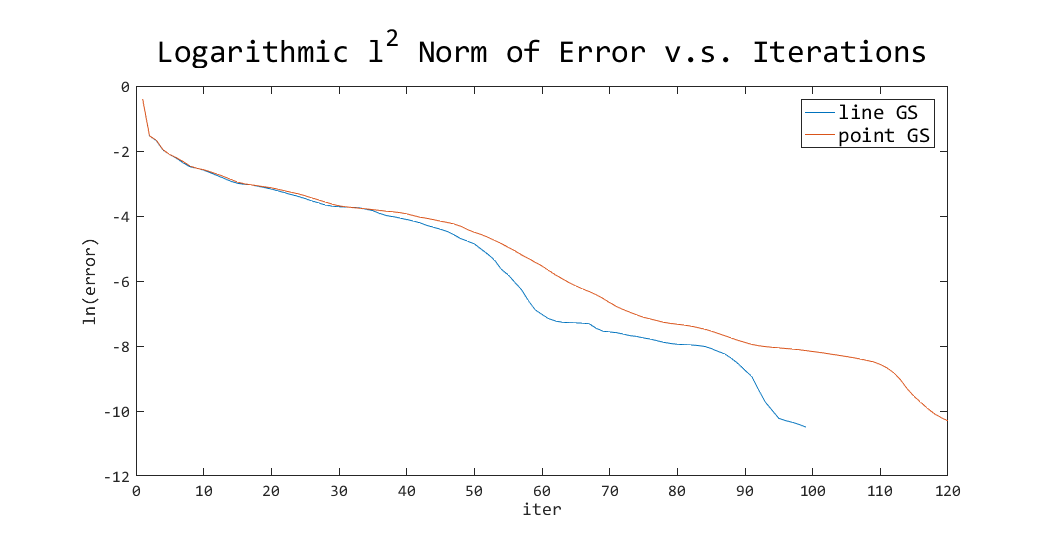
\includegraphics[width=\columnwidth]{error}}
\caption{The logarithmic $l^2$ norm of error of both line G-S iteration and point G-S iteration.}
\label{fig1}
\end{center}
\vskip -0.2in
\end{figure}

\section{Other Attempts}

Some other methods are attempted in the project.

Firstly, an ordinary conjugate gradient (CG) method is attempted. Surprisingly, despite thousands of iterations are implemented in the CG method and relatively poor performances when $\epsilon$ is large, the time costs of CG in some specific setups are the best among all other methods. Table~\ref{tab5} and Table~\ref{tab6} shows the time and iterations of the ordinary CG method. The variation of the times of iterations are similar to the one in the PCG + V-Cycle method.

\begin{table}[t]
\caption{The iterations of the ordinary CG method. Identical parameters and halt standard with Table~\ref{tab2}. }
\label{tab5}
\vskip 0.15in
\begin{center}
\begin{small}
\begin{sc}
\begin{tabular}{lrrrrrr}
\toprule
$N\backslash\epsilon$ & $10^0$ & $10^{-1}$ & $10^{-3}$ & $10^{-5}$ & $10^{-7}$ \\
\midrule
32 & 52 & 81 & 60 & 32 & 16 \\
64 & 102 & 158 & 157 & 64 & 32 \\
128 & 202 & 307 & 372 & 128 & 64 \\
256 & 396 & 593 & 760 & 256 & 128\\
512 & 771 & 1154 & 1442 & 754 & 257 \\
1024 & 1507 & 2208 & 2687 & 1939 & 1024 \\
\bottomrule
\end{tabular}
\end{sc}
\end{small}
\end{center}
\vskip -0.1in
\end{table}

\begin{table}[t]
\caption{The CPU time of the ordinary CG method. Identical parameters and halt standard with Table~\ref{tab2}. }
\label{tab6}
\vskip 0.15in
\begin{center}
\begin{small}
\begin{sc}
\begin{tabular}{lrrrrrr}
\toprule
$N\backslash\epsilon$ & $10^0$ & $10^{-1}$ & $10^{-3}$ & $10^{-5}$ & $10^{-7}$ \\
\midrule
32 & .01 & .00 & .00 & .00 & .00 \\
64 & .01 & .01 & .01 & .01 & .01 \\
128 & .07 & .11 & .11 & .04 & .03 \\
256 & .55 & .81 & 1.03 & .35 & .19\\
512 & 5.87 & 8.77 & 10.77 & 5.73 & 2.03 \\
1024 & 44.43 & 64.91 & 79.00 & 57.34 & 30.44 \\
\bottomrule
\end{tabular}
\end{sc}
\end{small}
\end{center}
\vskip -0.1in
\end{table}

Compared with Table~\ref{tab2}, it is obvious that the ordinary CG takes times more iterations to converge than the PCG + V-Cycle methods, and when $N$ and $\epsilon$ are large, the time cost of ordinary CG is way more than the PCG method. However, in some specific cases, the ordinary CG performs a lot better than the PCG method, especially the case when $N=1024$ and $\epsilon=10^{-7}$. 

Actually, the complexities of one iteration in ordinary CG and PCG + V-Cycle are both $O(N^2)$, while in the latter  the constants are way larger. Therefore, although the PCG + V-Cycle method is taking considerably less iterations, its large constants may sometimes lead to worse performance than the ordinary CG. The ordinary CG takes relatively less iterations when $\epsilon$ is rather small, and the decrease of iterations in the PCG method is not as obvious as the ordinary CG method. This is the direct reason for the situation described above.

Secondly, a naive PCG method is attempted. The naive PCG method takes the diagonal sub-matrices as the preconditioning matrix, i.e.
\begin{displaymath}
  M=
  \left(
    \begin{array}{ccccc}
      D & 0 & 0 & \cdots & 0 \\
      0 & D & 0 & \ddots & 0 \\
      0 & 0 & D & \ddots & 0 \\
      \vdots & \ddots & \ddots & \ddots & 0 \\
      0 & 0 & 0 & 0 & D
    \end{array}
  \right),
\end{displaymath}
where the inverse of D is pre-calculated (or an LU decomposition of D). The results show that\footnote{Detailed results are shown in Appendix 2. } the preconditioning only slightly reduces the iterations taking than an ordinary CG method, and the cost computing the triangular equation $Mz=r$ adds to the total cost of the method. Therefore, the method performs poorly than the methods described above.

\section{Conclusion}

In this project, various methods are conducted to solve the sparse linear equation $Au=f$. PCG + V-Cycle preconditioner + symmetric line Gauss-Seidel iterative smoother is a good combination to solve the problem, while in some special cases when $\epsilon$ is rather small, ordinary CG out-performs this method.

Comparing with the poor performance of the direct Gauss elimination method, it shows that an iterative method is usually better than a direct method in sparse problems. The experiment of the naive PCG shows the importance of choosing a good preconditioner is crucial in conducting the PCG method. A good preconditioner shall be easy to calculate, and significantly helpful in reducing the necessary iterations to convergent.

\end{document}
